\hypertarget{sec:5}{%
\section{Results}\label{sec:5}}

\hypertarget{sec:5-1}{%
\subsection{RQ1: Detection and Component Comparisons}\label{sec:5-1}}

Integrated App detects 105/126 controlled modifications with 0/252 controlled-normal alarms (Table~\ref{tab:app}). The refitted Web-only and no-memory alternatives each detect 96/126; all nine differences occur in the CPU-plus-memory recipe. No-timezone retains 105/126 because an absolute-offset condition substitutes on this benchmark. Removing the MTC cap adds three screen detections, whose normal-data cost appears in Section~\ref{sec:5-3}. The fixed App tree detects 72/126.

\ifHGMatrix\else
% Current manuscript Table 3. Source: input_markdown/sections/05_results.md.
\begin{table}[t]
  \caption{Controlled benchmark-position outcomes. All methods have zero U, FAILED, and EMPTY\_MODEL counts on these held-out positions. Ablations are separately refitted models.}
  \label{tab:app}
  \centering
  \small
  \setlength{\tabcolsep}{3pt}
  \renewcommand{\arraystretch}{1.12}
  \begin{tabularx}{\columnwidth}{@{}>{\raggedright\arraybackslash}p{0.28\columnwidth} *{4}{>{\centering\arraybackslash}X}@{}}
    \toprule
    Method & \makecell{Detected /\\modified} & \makecell{Detection\\(\%)} & Missed & \makecell{Normal\\alarms} \\
    \midrule
    Integrated App & 105/126 & 83.3 & 21 & 0/252 \\
    No MTC cap & 108/126 & 85.7 & 18 & 0/252 \\
    Web-only & 96/126 & 76.2 & 30 & 0/252 \\
    No memory & 96/126 & 76.2 & 30 & 0/252 \\
    No timezone & 105/126 & 83.3 & 21 & 0/252 \\
    App tree & 72/126 & 57.1 & 54 & 0/252 \\
    \bottomrule
  \end{tabularx}
\end{table}

\fi


All six methods miss 9/9 webdriver-only and 9/9 WebGL-identifier modifications. Historical raw WebGL unavailability and lost webdriver-false semantics limit the admission of their corresponding candidates. These misses expose gaps in the available feature representation and candidate-admission process for the tested edits. Appendix~\ref{app:main} describes the recipe grouping, and the supplemental tables retain all 84 recipe-by-method cells.

% Register the wide mechanisms figure and historical-normal table before the RQ2 text,
% retaining the approved visual assets while allowing page-seven placement.
\begin{figure*}[t]
  \centering
  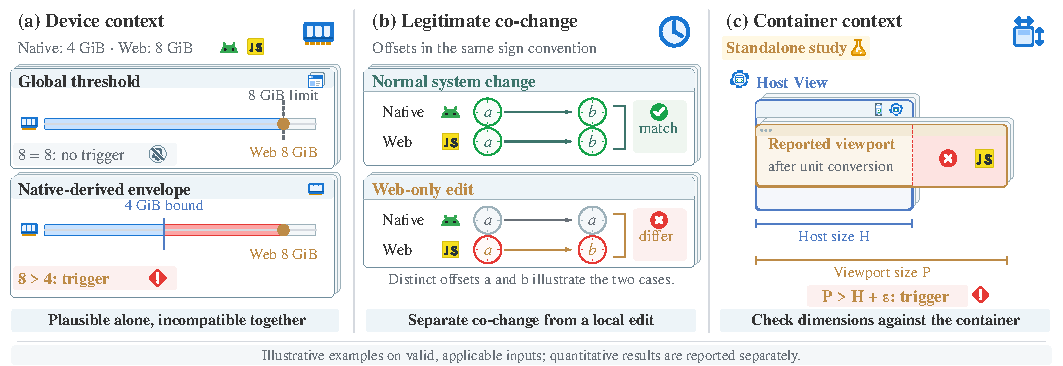
\includegraphics[width=\textwidth]{figures/HybridGuard_Fig3_mechanisms_v3.pdf}
  \caption{Illustrative mechanisms on applicable observations. (a) A Web report of 8 GiB stays within the fixed 8 GiB comparator but exceeds the envelope derived from Native memory of 4 GiB. (b) After offsets are converted to the same sign convention, a normal system change moves Native and Web together, whereas a Web-only edit creates a mismatch. (c) A converted viewport dimension P exceeding the Host bound plus tolerance triggers the standalone geometry check. These schematics add no measured records.}
  \label{fig:mechanisms}
  \Description{Three illustrative panels show a Native memory bound, legitimate timezone co-change versus a Web-only change, and a standalone Host geometry bound.}
\end{figure*}

% Table 5: single-column cohort groups; bars use the exact T/F/U proportions.
% Source: input_markdown/sections/05_results.md.
\begin{table}[t]
  \caption{Historical-normal decision counts by cohort. Entries report T (alarm), F (definite no alert), and U (unknown). Configurations 01 and 02 share identical per-model counts and one display row. FAILED and EMPTY\_MODEL are zero throughout.}
  \label{tab:normals}
  \centering
  \small
  \setlength{\tabcolsep}{4pt}
  \renewcommand{\arraystretch}{1.12}
  \begin{tabularx}{\columnwidth}{@{}l *{2}{>{\centering\arraybackslash}X}@{}}
    \toprule
    Config. & Integrated App & No cap \\
    \midrule
    \multicolumn{3}{@{}l}{\textbf{Historical development} ($N=144$)} \\
    01 / 02 & \makecell{1 / 135 / 8\\\HGOutcomeBar{1}{135}{8}{0.30\columnwidth}} & \makecell{144 / 0 / 0\\\HGOutcomeBar{144}{0}{0}{0.30\columnwidth}} \\
    03 & \makecell{0 / 136 / 8\\\HGOutcomeBar{0}{136}{8}{0.30\columnwidth}} & \makecell{144 / 0 / 0\\\HGOutcomeBar{144}{0}{0}{0.30\columnwidth}} \\
    \addlinespace[2pt]
    \multicolumn{3}{@{}l}{\textbf{Historically reserved} ($N=117$)} \\
    01 / 02 & \makecell{1 / 110 / 6\\\HGOutcomeBar{1}{110}{6}{0.30\columnwidth}} & \makecell{117 / 0 / 0\\\HGOutcomeBar{117}{0}{0}{0.30\columnwidth}} \\
    03 & \makecell{0 / 111 / 6\\\HGOutcomeBar{0}{111}{6}{0.30\columnwidth}} & \makecell{117 / 0 / 0\\\HGOutcomeBar{117}{0}{0}{0.30\columnwidth}} \\
    \bottomrule
  \end{tabularx}
  \par\smallskip
  \begin{minipage}{\columnwidth}\footnotesize
  Bars show the same T / F / U proportions: dark gray / light gray / outlined white. A fully dark bar means every normal record triggered an alarm.
  \end{minipage}
\end{table}


\hypertarget{sec:5-2}{%
\subsection{RQ2: What References Contribute}\label{sec:5-2}}

The specialist studies evaluate fixed checks separately from the fitted detectors to distinguish three mechanisms (Figure~\ref{fig:mechanisms}; Table~\ref{tab:specialists}). Their comparators use Web memory above 8 GiB, Web timezone offset above −480 minutes, and Web height above 710 CSS pixels. The fixed thresholds provide study-specific reference points for comparing the three semantic mechanisms. Appendix~\ref{app:5} describes their recorded freezing and the scope of these comparisons.

\textbf{Device-specific memory context.} The nine CPU-plus-memory positions separating Integrated App from the refitted alternatives also trigger the fixed 8 GiB check. That main-benchmark difference alone does not establish the need for a device-specific reference. The memory specialist supplies the distinction: the Native envelope detects 18/18 modifications, versus 6/18 for the global threshold, with 0/48 normal alarms for both. Its twelve additional detections are upward edits to 4 and 8 GiB; both checks detect six edits to 16 GiB. Neither triggers on the six no-effect operations targeting 2 GiB. These twelve specialist detections are separate from the nine App-model differences and concern the tested upward edits.

\textbf{Legitimate timezone co-change.} Both checks detect 6/6 modifications. The absolute-offset check also alarms on six normal system changes; the Native reference avoids those alarms. Thus, unchanged main-benchmark detection after removing Native timezone hides a difference in handling legitimate changes. Modification totals alone do not expose this benefit.

\textbf{Host container context.} The fixed Web-height check detects 6/6 modifications but alarms on 6/66 normals. The same-Web viewport relation avoids normal alarms yet misses all six modifications. The Host bound achieves 6/6 detection and 0/66 alarms. This standalone result does not describe Integrated App: configurations 01/02 retain the old height check and alarm on the six normal layout changes, while configuration 03 misses the six modifications. Integrating the Host specialist requires a separate model-construction evaluation.

\hypertarget{sec:5-3}{%
\subsection{RQ3: Normal Alarms and Unavailable Evidence}\label{sec:5-3}}

Removing the historical-normal alarm cap raises controlled detection from 105 to 108 but alarms on every record in both historical groups (Table~\ref{tab:normals}). Both alternatives have 0/252 controlled-normal alarms, so the controlled benchmark alone conceals this cost. Saved uncapped models include broad conditions such as hardware concurrency greater than one and language-list length greater than one. The controlled-normal budget alone does not adequately constrain these checks on MTC records.

On the separate 630 training normals, Integrated App configurations 01/02/03 produce 6/6/0 alarms and 51 unknowns each; uncapped models alarm on all 630. We keep these training outcomes separate from evaluation. Each Integrated App configuration yields 14/261 unknowns across the two historical evaluation groups. Removing memory reduces that count to 1/261 but also loses resource detections. A tree can return a definite label when some candidate states are unknown, because its traversed path need not use those candidates.

\hypertarget{sec:5-4}{%
\subsection{RQ4: Increment from a Linked Browser}\label{sec:5-4}}

On the 60 paired App--Browser positions used during extension development (14 effective modifications and 46 normals), adding C1 raises detection from 2/14 to 7/14 (Table~\ref{tab:paired}). All five additional detections arise from Browser timezone edits; App timezone detection remains 2/2, while the tested App and Browser language edits remain undetected. Both configurations yield 0/46 normal alarms. These aggregate counts hold for each of the three frozen App models and are presented once for the shared 60-position set.

% Table 6: detection symbols apply to modifications, never the normal-alarm row.
% Source: input_markdown/sections/05_results.md.
\begin{table}[t]
  \caption{Paired App--Browser outcomes with development-use history. App = Integrated App; T counts detected modifications or normal alarms. U and FAILED are zero.}
  \label{tab:paired}
  \centering
  \small
  \setlength{\tabcolsep}{3pt}
  \renewcommand{\arraystretch}{1.12}
  \begin{tabularx}{\columnwidth}{@{}>{\raggedright\arraybackslash}X c >{\centering\arraybackslash}p{0.25\columnwidth} >{\centering\arraybackslash}p{0.29\columnwidth}@{}}
    \toprule
    Record family & $N$ & App: T & App + C1: T \\
    \midrule
    App timezone & 2 & \HGFull\,2 & \HGFull\,2 \\
    App language & 2 & \HGNone\,0 & \HGNone\,0 \\
    Browser timezone & 5 & \HGNone\,0 & \HGFull\,5 \\
    Browser language & 5 & \HGNone\,0 & \HGNone\,0 \\
    \midrule
    Normal alarms & 46 & 0 & 0 \\
    \bottomrule
  \end{tabularx}
  \par\smallskip
  \begin{minipage}{\columnwidth}\footnotesize
  Modification rows: \HGFull\ all $N$ detected; \HGNone\ none detected.
  \end{minipage}
\end{table}


C1 also raises historical unknowns from 8/144 to 11/144 in development, while leaving 6/117 in the historically reserved group. The combined count increases from 14/261 (5.4\%) to 17/261 (6.5\%) per model, with unchanged alarms. Asynchronous legitimate timezone changes remain an untested operating condition for C1's timestamp-independent offset comparison. The paired language tests cover App- and Browser-side report edits; the App benchmark separately evaluates a Web language-list modification recipe. C1 provides a targeted increment for the tested timezone edits, accompanied by lower definite-output coverage.
